% IzPack - Documentation

% User Input

\chapter{\label{chap:userinput}User Input} (by Elmar \textsc{Grom})\\

Most of the panels that come with IzPack take user input in some form.
In some panels this is through a simple user acknowledgement in others
the user can enter text or select a directory thorugh a file open
dialog. In all of those cases the user input is used for the specific
purpose  needed by the panel that takes the input. However, if you need
user input during installation that will later on be available  to your
application then you need to use the user input panel.\\

{\sloppy To use this panel list it in the install file with the class name
\texttt{UserInputPanel}. In addition you must write a XML specification
and add it to the install resources. The name of this resource must be
UserInputSpec.xml.}

The user input panel is a blank panel that can be populated with UI
elements through a XML specification file. The specification supports
text labels, input elements, explanatory text and some minor formatting
options.\\

The following types of user input elements are supported:
\begin{itemize}
\item Text
\item Combo Box
\item Radio Buttons
\item Check Box
\item Rule Input Field
\item Search Field
\end{itemize}\

The way in which this panel conveyes the user input to your application
is through the variable substitution system. User input is not directly
inserted into your configuration files but the variables that you
specify for this panel are set in the variable substitution system.
After this operation has taken place the variables and associated values
are available for all substitutions made. This way of operation has a
number of implications that you should be aware of.\\

First, not only can you set additional variables in this way but you can
also modify variables that are defined elsewhere -even built in
variables. For this reason you should be careful to avoid overlaps when
chosng variable names. Although there might be cases when it seems
useful to modify the value of other variables, it is generally not a
good idea to do so. Because you might not exactly know when other
variables are set and when and where they are used throughout the
installation process, there might be unintended side effects.\\

Second, the panel must be shown at a point during the installation
process before the variables are used. In most cases you will use the
values to substitute variables in launch and configuration files that
you supply with your installation. For this to work you place this panel
before the install panel, because the install panel uses the variable
substitutor to replace all such variables. Although using this panel any
later in the process will correctly set the variables internally, there
won't be any affect on the files written to disk. You can also use
variables set in this way in other panels that you have written
yourself. There is a section in the  chapter on writing your own panel
that explains how to do this. Also in this case it is important to place
the associated input panel in the process before the variables are
used.\\

At this point I would also like to mention that it is possible to hide
select elements on the panel or the panel altogether if certain packs
are not selected. For this to work you must place this panel after the
packs panel. One side effect of using this feature is that it is not
possible to step back once the user input panel is displayed. This is
because the user might make changes in the packs selection that would
require a complete rebuild of the UI. Unfortunatly, building the UI is
an irreversible process, therefore the user can not be allowed to go
back to the packs panel.\\


\section{The Basic XML Structure}

The top level XML section is called \texttt{<userInput>}. For most
panels it does not make sense to present them more than once, however
you might want to present multiple user input panels -with different
content of course. Therefore the \texttt{<userInput>} section can
contain multiple tags that each specify the details for one panel
instance. The tag name for this is \texttt{<panel>}.\\

The \texttt{<panel>} tag uses the following attributes:\\

\textbf{order} \texttt{- required}\\

This is the order number of the user input panel for which this
specification should be used. Counting starts at 0 and increments by 1
for each instance of the user input panel. So if a spec should be used
for the second occurrence of the user input panel use
\texttt{order="1"}.\\

\textbf{layout} \texttt{- optional}\\

There are three general layout rules this panel uses, they are
\texttt{left}, \texttt{center} and \texttt{right}. While I think left is
most commonly used, you might want to experiment with this attribute and
see which you like best. The default is \texttt{left}.\\


\section{Concepts and XML Elements Common to All Fields}

Before I dive into the details of defining the various UI elements I
would like to present XML elements and general concepts that apply
thoughout. This saves me a lot of work in writing and you a lot of
repetitive reading and maybe a tree or two.\\

The UI elements are generally laid out top to bottom in the order they
appear in the XML file. The only exception to this rule is the title,
which always appears at the very top. The layout pattern for the input
fields is as follows: If a description is defined, it appears first,
using the full available layout width. The input field is placed beneath
the description. With fileds such as the text filed or the combo box,
the label is placed to the left and the input field to the right. Fields
such as radio buttons and check boxes are somewhat indented and have the
label text appear to their right.\\

Each UI element is specified with a \texttt{<field>} tag. The
\texttt{type} attribute is used to specify what kind of field you want
to place. Obviously, the \texttt{type} attribute is not optional.\\

Each field that takes user input must also specify the variable that
should be substituted. This is done with the \texttt{variable}
attribute.\\

\label{userInput:descriptiontag}
Almost all fields allow a description. When a description is allowed it
is always added in the same way. The description is part of the data
within the field tag. There can only be one description per field. If
you add more than one, the first one is used and the others ignored.
There are three attributes used with this tag. The text is specified
through the \texttt{txt} or the \texttt{id} attribute. The details on
using them are described below. The attributes are all optional but you
must specify text to use, either directly or through the \texttt{id}
attribute. In addition, you can set the text justification to
\texttt{left}, \texttt{center} and \texttt{right} with the
\texttt{align} attribute. \\

The following example illustrates the general pattern for field specification:\\

\footnotesize
\begin{verbatim}
<field type="text" variable="myFirstVariable">
  <description align="left" txt="A description" id="description 1"/>
  .
  .
  .
</field>
\end{verbatim}
\normalsize

A very frequently used pattern is for the definition of text. Where ever
text is needed (lables, descriptions, static text, choices etc.) it can
be specified in place using the \texttt{txt} attribute. This is
conveninet if you are only supporting a single language. However, if you
would like to separate your text definitions from the panel
specification or if you need to support multiple languages you might
want to use the \texttt{id} attribute instead to only specify an
identifier. You can then add multiple XML files with the same name as
this spec file (UserInputSpec.xml) appended with an unserscore '\_' and
the the appropriate three letter ISO3 language code. The content of
those files must conform to the specification for IzPack language
packages. For more details on this topic see the chapter on language
packages under advanced features. \texttt{id} defines an identifier that
is also defined in the language package, toghether with the localized
text to use. It is possible to use both the \texttt{txt} and the
\texttt{id} attribute. In this case the text from the language package
is used. If for some reason the language package is not available or the
\texttt{id} is not defined there, the text specified with \texttt{txt}
is used as default.\\

All input fields can be pre-set with a value of your choice. Although
the details vary a bit from field type to field type, the \texttt{set}
attribute is always used to accomplish this. The \texttt{set} attribute
is of course optional.\\

All fields that take user input use a \texttt{<spec>} tag to define the
details of the input field. In the some cases the content of this tag is
rather simple. Input fields with a more complex nature tend to have
accordingly complex content in this tag. Since the details vary widely,
they are explained with each input field.\\

Any number of \texttt{<createForPack>} tags can be added to the
\texttt{<panel>} and \texttt{<field>} sections. This tag has only one
attribute and no data. The attribute is \texttt{name} and specifies the
name of one of the installation packs that you have defined. Here is how
it works: if no \texttt{<createForPack>} tag exists in a section, the
entity is always created. However, if the tag exists, the entity is only
created if one or more of the listed packs are selected for
installation. As mentioned before, if you are using this feature, make
sure the user input panel shows up after the packs panel.\\

\section{Panel Title}

You can place an optional title at the top of the panel. Though it is
not possible to select a font for the title that is different form the
one used on the rest of the panel, it is possible to modify the font to
some extent. To specify the title create a \texttt{<field>} tag and use
the \texttt{type} attribute with the value \texttt{title}. In addition
to the \texttt{txt} and \texttt{id} attributes, the following attributes
are supported:\\

\textbf{italic} \texttt{- optional}\\

With a value of \texttt{true} specifies that the title font should be in italics.\\

\textbf{bold} \texttt{- optional}\\

With a value of \texttt{true} specifies that the title font should be bold.\\

\textbf{size} \texttt{- optional}\\

This attribute specifies the size of the title font. Please note that
the size is not sprcified in points but as a relative size multiplier
compared to the body font on the panel. The default value is 2.\\

\section{Static Text}

Static text is simply text that is placed on the panel without direct
connection to any of the input elements. It is laid out to use the
entire layout width available on the panel and is broken into multiple
lines if necessary. To specify static text create a \texttt{<field>} tag
and use the \texttt{type} attribute with a value of \texttt{staticText}.
In addition to the \texttt{txt} and \texttt{id} attributes, the text can
be justified \texttt{left}, \texttt{center} or \texttt{right} with the
\texttt{align} attribute. It is not possible to format this text in any way.\\

\textbf{Example}\\

The following example inserts some static text in the panel.

\footnotesize
\begin{verbatim}
<field type="staticText" align="left" 
       txt="This is just some simple static text."
       id="staticText.text"/>
\end{verbatim}
\normalsize

\section{Visual Separation}

Sometimes it is desirable to separate different entities visually. This
can be accomplished by inserting a space or a divider. A space simply
inserts a vertical separation of the average height of a single line
lentity, such as a line of text or a an input field. A divider inserts
the same amout of space but also draws a division line which can be
either aligned at the top or bottom of the separation.
\texttt{<space>}, \texttt{<divider>}

 ..... maybe I should draw the line myself and add no additional space at all ...

\section{Text Input}

A text input field allows the user to enter and edit a single line of
text, without lenght restriction. The input field can have a label,
which will show to the left of the input field and a description, which
can span multiple lines. The description is placed above the input field
and uses the entire available layout width. The width of the input field
must be explicitly set, otherwise it will only accomodate a single
character. To specify a text input field create a \texttt{<field>} tag
and use the \texttt{type} attribute with a value of \texttt{text}. The
\texttt{txt} and \texttt{id} attributes are not supported here. The
\texttt{variable} attribute specifies the variable that should be
replaced with the text taken from the input field.\\

\textbf{The Data}\\

The data consists of two items, a description and the spec. The
\texttt{<spec>} tag uses four attributes. The label text is specified with
\texttt{txt} and/or \texttt{id} as described above. In addition, the
width of the input field as it appears on the panel can be set with the
\texttt{size} attribute. The value must be an integer and sets the field
width based on the average character width of the active font. If this
is not specified, then you will end up with a very narrow field that is
practically unusable.\\

The fourth attribute \texttt{set} is optional. It takes a text string to
pre-fill the input field.\\

\textbf{Example}\\

The following example creates a text input field with a label and
description. The width of the input field will be enough to accommodate
15 characters. The field will be pre-set with the text 'some text' when
the UI is first presented.\\

\footnotesize
\begin{verbatim}
<field type="text" variable="textInput">
  <description align="left" txt="A description for a text input field"
               id="description.text"/>
  <spec txt="Enter some text:" id="text.label" size="15" set="some text"/>
</field>
\end{verbatim}
\normalsize

\section{Radio Buttons}

The radio buttons are useful when the user needs to select a specific
option out of a pre-defined list of choices. This field offers an
arbitrary number of mutually exclusive buttons, each with its own label.
The placement of the buttons and labels is different form other fields.
First, the button is placed to the left and the label text to the right.
Second, the buttons are not lined up all the way to the left as other
lables are but they are indented from that location. As with other
fields, the description is placed above the list of radio buttons and
uses the entire available layout width. To specify a set of radio
buttons create a \texttt{<field>} tag and use the \texttt{type}
attribute with a value of \texttt{radio}. The \texttt{txt} and
\texttt{id} attributes are \textbf{not} supported here. As with all
other input fields, the \texttt{variable} attribute specifies that
variable that should be replaced with the user selection.\\

\textbf{The Data}\\

The data consists of two items, a description and the spec. The
\texttt{<spec>} tag has no attributes, instead the specification details
are entered as data within the \texttt{<spec>} tag. The \texttt{<spec>}
data consists of one or more \texttt{<choice>} tags. One
\texttt{<choice>} tag is required for each radio button. The
\texttt{<choice>} tag accepts the usual \texttt{txt} and \texttt{id}
attributes, which are used to specify the label text. In addition the
following attributes are supported:\\

\textbf{value} \texttt{- required}\\

The \texttt{value} attribute is used to specify which value to insert if
this associated radio button is selected. In other words, the label text
has nothing to do with the value that is actually substituted for the
variable. For this reason there is never an issue if multiple languages
are used, the value is always the same for a given selection.\\

\textbf{set} \texttt{- optional}\\

The \texttt{set} attribute accepts the values \texttt{true} and
\texttt{flase}. Since the attribute is optional it can also be omitted,
which is interpreted as \texttt{false}. If a value of \texttt{true} is
used, the associated radio button will be selected when the UI is first
presented. Obviously, only one of the buttons in a set should be set to
\texttt{true}.\\

\textbf{Example}\\

The following example creates a set of four radio buttons with
description. The second button will be selected when the UI is first
presented.\\

\footnotesize
\begin{verbatim}
<field type="radio" variable="radioSelection">
  <description align="left" txt="This is a description for radio buttons"
               id="description.radio"/>
  <spec>
  <choice txt="the first choice" id="radio.label.1" value="1 selected" />
  <choice txt="the second choice" id="radio.label.2" value="2 selected"
          set="true" />
  <choice txt="the third choice" id="radio.label.3" value="3 selected" />
  <choice txt="the fourth choice" id="radio.label.4" value="4 selected" />
  </spec>
</field>
\end{verbatim}
\normalsize

\section{Combo Box}

The combo box provides essentially the same functionality as do the
radio buttons, just in a different presentation stile. The advantage of
the combo box is that it is easier to deal with a long list of
choices.\\

\section{Check Box}

If there are a number of choices and any combination of them could be
selected, not just a single one, then radio buttons are not the way to
go. You might be better off using a number of check boxes. The layout
for a check box works in the same way as for radio buttons. The check
box is placed indented from the left most edge and the label text is
placed to the right of it. Other than with radio buttons, you cannot
define any number of check boxes. This field allows the definition of
only one check box, which is associated with one variable. If you need
multiple check boxes you need to define one field for each of them.  To
make it look like a cohesive group you simply provide a description only
for the first check box. All of the check boxes will be positioned in
such a way that they look like a group, even though they are separate
entities and their selections are conveyed to different variables. The
description  is placed above the check box and uses the entire available
layout width. To specify a check box create a \texttt{<field>} tag and
use the \texttt{type} attribute with a value of \texttt{check}. As with
all other input fields, the \texttt{variable} attribute specifies the
variable that should be replaced with the user input.\\

\textbf{The Data}\\

The data consists of two items, a description and the spec. The
\texttt{<spec>} tag accepts the usual \texttt{txt} and \texttt{id}
attributes, which are used to specify the label text. In addition, the
following attributes are supported:\\

\textbf{true} \texttt{- required}\\

The \texttt{true} attribute specifies the value to use for substitution
when the box is selected.\\

\textbf{false} \texttt{- required}\\

The \texttt{false} attribute specifies the value to use for substitution
when the box is not selected.\\

\textbf{set} \texttt{- optional}\\

The \texttt{set} attribute accepts the values \texttt{true} and
\texttt{flase}. Since the attribute is optional it can also be omitted,
which is interpreted as \texttt{false}. If a value of \texttt{true} is
used, the check box will be selected when the UI is first presented.\\

\textbf{Example}\\

The following example creates a check box with description. The check
box will not be selected when the UI is first presented. This could also
be accomplished by ommitting the \texttt{set} attribute.\\

\footnotesize
\begin{verbatim}
<field type="check" variable="chekSelection.1">
  <description align="left" txt="This is a description for a check box"
               id="description.check.1"/>
  <spec txt="check box 1" id="check.label.1" true="on" false="off" 
        set="false"/>
</field>
\end{verbatim}
\normalsize

\section{Rule Input}

The rule input field is the most powerful and complex one of all the
input fields offerd by this panel. In its most simple incarnation it
looks and works like a regular text input field. There is also only an
incremental increase of the complexity in the specification for this
case. However, it is unlikely that you would use it for such a purpose.
The real power of this input field comes from the fact that rules can be
apllied to it that control many aspects of its look as well as overt and
covert operation.\\

\subsection{Layout and Input Rules}

The basic nature of this input field is that of a text input field and
as mentioned before, in its most simple incarnation that is what it
looks like and how it operates. However, the layout of the field can be
defined in such a way that there are multiple logically interconnected
text input fields, adorned with multiple labels. Further more, each of
these fields can be instructed to restrict the type of input that will
be accepted. Now you might ask what this could be useful for. As an
answer, let me present a few examples that show how this feature can be
used. Before I do this howerver, I would like to describe the
specification syntax, so that the examples can be presented together
with the specifactions that make them work in a meaningful way.\\

The actual specification of the layout, the lables and the type of input
each field accepts all happens in a single string with the
\texttt{layout} attribute. First let us have a look at the specification
format for a single field. This format consists of a triplet of
information, separated by two colons ':'. A typical field spec would
look like this: \texttt{N:4:4}, where the first item is a key that
specifies the type of input this particular field will accept - numeric
input in the example. The second item is an integer number that
specifies the physical width of the field, this is the same as in the
with of any regular text field. Therefore the field in the example will
provide space to display four characters. The third item specifies the
editing length of the string or in other words, the maximum length of
the string that will be accepted by the field. In the \texttt{layout}
string you can list as may fields as you need, each with its own set of
limitations. In addition you can add text at the front, the end and in
between the fields. The various entities must be separated by white
space. The behavior of this field is such that when the editing length
of a field has been reached, the cursor automatically moves on to the
next field. Also, when the backspace key is used to delete characters
and the beginning of a field has been reached, the cursor automatically
moves on to the previous field. So let us have a look a some examples.\\

\textbf{Phone Number}

The following specification will produce a pre formatted input field to
accept a US phone number with in-house extension. Even though the
pattern is formatted into number groups as customary, complete with
parentheses '(' and dash '-', entering the number is as simple as typing
all the digits. There is no need to advance using the tab key or to enter
formatting characters. Because the fields only allow numeric entry, there
is a much reduced chance for entering erroneous information.
\texttt{"( N:3:3 ) N:3:3 - N:4:4 x N:5:5"}. Each of the fields uses the
'N' key, indicating that only numerals will be accepted. Also, each of
the fields only accepts strings of the same length as the physical width
of the field.\\

\begin{center}
\fbox{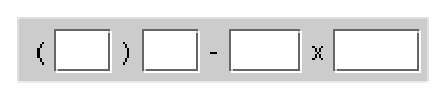
\includegraphics[scale=1.0]{img/userInput-phone}}
\end{center}

\textbf{E-Mail Adress}

This specification creates a pattern that is useful for entering an
e-mail address \texttt{"AN:15:U @ AN:10:40 . A:4:4"}. Even though the
first field is only fifteen characters wide it will accept a string of
unlimited length, because the 'U' identifier is used for the edit
length. The second field is a bit more restrictive by only accepting a
string up to fourty characters long.\\

\begin{center}
\fbox{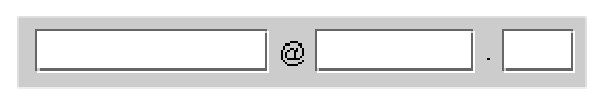
\includegraphics[scale=1.0]{img/userInput-email}}
\end{center}

\textbf{IP Address}

It might not be uncommon to require entering of an IP address. The
following simple specification will produce the necessary input field.
All fields are the same, allowing just three digits of numerical entry.
\texttt{"N:3:3 . N:3:3 . N:3:3 . N:3:3"}\\

\begin{center}
\fbox{
\includegraphics[scale=1.0]{img/userInput-IP}}
\end{center}

\textbf{Serial Number or Key Code}

If you ship your product with a CD key code or serial number and require
this information for registration, you might want to ask the cutomer to
trasncribe that number from the CD label, so that it is later on
accessible to your appication. As this is always an error prone
operation, the predefined pattern with the easy editing support and
restriction of accepted data helps to reduce transcription errors
\texttt{"H:4:4 - N:6:6 - N:3:3"}. This particular specification will
produce three fields, the first accepting four hexadecimal, the second
six numerical and the third three numerical digits.\\

\begin{center}
\fbox{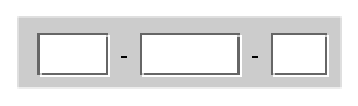
\includegraphics[scale=1.0]{img/userInput-serial}}
\end{center}

\textbf{Limitations}

Even though the above examples all use single character lables between
fields, there is no restriction on the length of these lables. In
addition, it is possible to place label text in front of the first field
and after the last field and the text can even contain spaces. The only
limitation in this regard is the fact that all white space in the text
will be reduced to a single space on the display. This means that it is
not possible to use multiple spaces ot tabs in the text.\\

The following table lists and describes all the keys that can be used in
the specification string.\\

\begin{center}
\begin{tabularx}{\textwidth}{|l|l|X|}
\hline \textit{Key} & \textit{Meaning} & \textit{Description} \\
\hline N & numeric & The field will acept only numerals.\\
\hline H & hexadecimal & The field will accept only hexa-decimal numerals, that is all numbers from 0-F.\\
\hline A & alphabetic & The field will accept only alphabetic characters. Numerals and punctuation marks will not be accepted.\\
\hline AN & alpha-numeric & The field will accept alphabetic characters and numerals but no punctuation marks.\\
\hline O & open & The filed will accept any input, without restriction.\\
\hline U & unlimited & This key is only legal for specifying the editing length of a fields. If used, the field imposes no length restriction on the text entered.\\
\hline
\end{tabularx}\
\end{center}

\subsection{Setting Field Content}

Like all other input fields the rule input field can also be pre-filled
with data and as usual, this is accomplished thought the \texttt{set}
attribute. As you might expect, the details of setting this field are
rather on the complicated side. In fact you can set each sub field
individually and you can leave some of the fields blank in the process.
The \texttt{set} specification for all sub fields is given in a single
string. Each field is addressed by its index number, with the count
starting at 0. The index is followed by a colon ':' and then by the
content of the field. The string "0:1234 1:af415 3:awer" would fill the
first subfield with \texttt{1234}, the scond one with \texttt{af415} and
the fourth with \texttt{awer}. The third subfield would stay blank
and so would any additional fields that might follow.\\

The individual field specs must be separated with spaces. Spaces within
the prefill values are not allowed, otherwise the result is undefined.\\

\subsection{The Output Format}

The user input from all subfields is combined into one single value and
used to replace the variable associated with the field. You can make a
number of choices when it comes to the way how the subfield content is
combined. This is done with the \texttt{resultFormat} and
\texttt{separator} attributes. The \texttt{resultFormat} attribute can
take the following values:\\

\begin{center}
\begin{tabularx}{\textwidth}{|l|X|}
\hline \textit{Value} & \textit{Meaning}\\
\hline \texttt{plainString} & The content of all subfields is simply concatenated into one long string.\\
\hline \texttt{displayFormat} & The content of all subfields and all lables -as displayed- is concatenated into one long string.\\
\hline \texttt{specialSeparator} & The content of all subfields is concatenated into one string, using the string specified withe the \texttt{separator} attribute to separate the content of the subfields.\\
\hline \texttt{processed} & The contnet is processed by Java code that you supply before replacing the variable. How to do this is discribed below.\\
\hline
\end{tabularx}\
\end{center}

\subsection{Validating the Field Content}

This feature needs to be documented.

\subsection{Processing the Field Content}

This feature needs to be documented.

\subsection{Summary Example}

\footnotesize
\begin{verbatim}
<field type="rule" variable="test1">
  <description align="left" txt="A description for a rule input field."
               id="description.rule.1"/>
  <spec txt="Please enter your phone number:" 
        layout="( N:3:3 ) N:3:3 - N:4:4 x N:5:5" 
        resultFormat="specialSeparator" separator="."/>
  <validator class="com.izforge.izpack.util.NotEmptyValidator"
             txt="The phone number is mandatory!" />
  <!--processor class=""/-->
</field>
\end{verbatim}
\normalsize

\section{Search}

The search input field allows the user to choose the location of files or
directories. It also supports autodetection of the location using a list of 
suggestions. The field is basically a combobox with an extra button to
trigger autodetection (again).

\begin{center}
\fbox{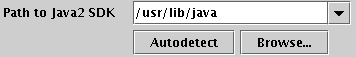
\includegraphics[scale=0.8]{img/userInput-search}}
\end{center}

\subsection{Specification}

The \texttt{<description>} tag is the same as with other fields (see
\ref{userInput:descriptiontag} on page \pageref{userInput:descriptiontag}). The
\texttt{<spec>} tag supports the following attributes:

\begin{itemize}
\item \texttt{filename} - the name of the file or directory to search for
\item \texttt{type} - what to search for
  \begin{itemize}
  \item \texttt{file} - search for a file
  \item \texttt{directory} - search for a directory
  \end{itemize}
\item \texttt{result} - what to return as the search result
  \begin{itemize}
  \item \texttt{file} - result of search is whole pathname of file or directory found
  \item \texttt{directory} - only return directory where the file was found (this is the same as \texttt{file} when searching for directories)
  \item \texttt{parentdir} - return the full path of the parent directory where the file was found
  \end{itemize}
\item \texttt{checkfilename} - the name of a file or directory to check for existence (this can be used to validate the user's selection)
\end{itemize}

\subsection{Example}

\footnotesize
\begin{verbatim}
<field type="search" variable="java_sdk_home">
  <description align="left" 
               txt="This is a description for a search input field."
               id="description.java_sdk_home"/>
  <spec txt="Path to Java SDK:" checkfilename="lib/tools.jar"
        type="file" result="directory">
  <choice value="/usr/lib/java/" os="unix" />
  <choice value="/opt/java" os="unix" />
  <choice value="C:\Program Files\Java" os="windows" />
  <choice value="C:\Java" os="windows" />
  </spec>
</field>
\end{verbatim}
\normalsize
